\documentclass[14pt,aspectratio=1610]{beamer}

\usepackage[brazil]{babel}
\usepackage[utf8]{inputenc}
%\UseRawInputEncoding
\usepackage[T1]{fontenc}
\usepackage{Sweave}
\usepackage{animate}
\usepackage{amsbsy}
\usepackage{amsfonts}
\usepackage{amsmath}
\usepackage{amssymb}
\usepackage{amsthm}
\usepackage[toc,page,title,titletoc]{appendix}
\usepackage[fixlanguage]{babelbib}
%\usepackage[pdftex]{color}
\usepackage{dsfont}
\usepackage{esvect}
\usepackage[labelfont=bf]{caption}
\usepackage{float}
\usepackage[Glenn]{fncychap}%Sonny %Conny %Lenny %Glenn %Renje %Bjarne %Bjornstrup
%\usepackage{geometry, calc, color, setspace}%
%\geometry{a4paper, headsep=1.0cm, footskip=1cm, lmargin=3cm, rmargin=2cm, tmargin=3cm, bmargin=2cm}
\usepackage{graphicx}
\usepackage{indentfirst}%Para indentar os parágrafos automáticamente
\usepackage{lipsum}
\usepackage{longtable}
\usepackage{mathtools}
\usepackage{listings}%Inserir codigo do R no latex
\usepackage{multirow}
\usepackage{multicol}
\usepackage{natbib}
\bibliographystyle{abbrvnat3}
\usepackage[figuresright]{rotating}
\usepackage{spalign}
%\usepackage{pgfpages}
\usepackage{pgfplots}
\usepackage{tikz}
\usepackage{color, colortbl}
\usepackage{ragged2e}%para justificar o texto dentro de algum ambiente
\definecolor{Gray}{gray}{0.9}
\definecolor{LightCyan}{rgb}{0.88,1,1}


\usepackage[all]{xy}
\usepackage{hyperref,bookmark}
\hypersetup{
  colorlinks=true,
  linkcolor=blue,
  citecolor=red,
  filecolor=blue,
  urlcolor=blue,
}

\usetheme{Boadilla}
%\usecolortheme[RGB={193,0,0}]{structure}

%\setbeamertemplate{footline}[frame number]
%\setbeamertemplate{footline}[text line]{%
%  \parbox{\linewidth}{\vspace*{-8pt}\hfill\date{}\hfill\insertshortauthor\hfill\insertpagenumber}}
\beamertemplatenavigationsymbolsempty
\renewcommand{\vec}[1]{\mbox{\boldmath$#1$}}
\newtheorem{Teorema}{Teorema}
\newtheorem{Proposicao}{Proposição}
\newtheorem{Definicao}{Definição}
\newtheorem{Corolario}{Corolário}
\newtheorem{Demonstracao}{Demonstração}
\newcommand{\bx}{\ensuremath{\bar{x}}}
\newcommand{\Ho}{\ensuremath{H_{0}}}
\newcommand{\Hi}{\ensuremath{H_{1}}}


\apptocmd{\frame}{}{\justifying}{} % Allow optional arguments after frame.

\title{MAF 261 - Estatística Experimental}
\author{Prof. Fernando de Souza Bastos}
\institute{Instituto de Ciências Exatas e Tecnológicas\texorpdfstring{\\ Universidade Federal de Viçosa}{}\texorpdfstring{\\ Campus UFV - Florestal}{}}
\date{2018}
\newcommand\mytext{Aula 8}
\newcommand\mytextt{Fernando de Souza Bastos}
\makeatletter
\setbeamertemplate{footline}
{
  \leavevmode%
  \hbox{%
  \begin{beamercolorbox}[wd=.333333\paperwidth,ht=2.25ex,dp=1ex,center]{author in head/foot}%
    \usebeamerfont{author in head/foot}\mytext
  \end{beamercolorbox}%
  \begin{beamercolorbox}[wd=.333333\paperwidth,ht=2.25ex,dp=1ex,center]{title in head/foot}%
    \usebeamerfont{title in head/foot}\mytextt
  \end{beamercolorbox}%
  \begin{beamercolorbox}[wd=.333333\paperwidth,ht=2.25ex,dp=1ex,right]{date in head/foot}%
    \usebeamerfont{date in head/foot}\insertshortdate{}\hspace*{2em}
    \insertframenumber{} / \inserttotalframenumber\hspace*{2ex} 
  \end{beamercolorbox}}%
  \vskip0pt%
}
\makeatother


\providecommand{\arcsin}{} \renewcommand{\arcsin}{\hspace{2pt}\textrm{arcsen}}
\providecommand{\sin}{} \renewcommand{\sin}{\hspace{2pt}\textrm{sen}}
%\newtheorem{Teorema}{Teorema}
%\newtheorem{Proposicao}{Proposição}
%\newtheorem{Definicao}{Definição}
%\newtheorem{Corolario}{Corolário}
%\newtheorem{Demonstracao}{Demonstração}

% Layout da pagina
\hypersetup{pdfpagelayout=SinglePage}
\begin{document}
\Sconcordance{concordance:Aula13.tex:Aula13.Rnw:%
1 339 1}


\frame{\titlepage}

\begin{frame}{}
\frametitle{\bf Sumário}
\tableofcontents
\end{frame}

\section{Delineamento em Blocos Casualizados}
\begin{frame}{Delineamento em Blocos Casualizados}
\frametitle{}
\begin{block}{}
\justifying
O delineamento inteiramente casualizado pressupõe para ser utilizado que, as
unidades experimentais sejam e estejam durante todo o experimento em condições
ambientais completamente homogêneas. Caso o pesquisador perceba que algum fator
perturbe a homogeneidade das unidades experimentais ou nas condições ambientais que
as mesmas vão estar sujeitas durante o experimento, é necessário que o pesquisador
controle o efeito deste fator pertubador.

\end{block}
\end{frame}

\begin{frame}{}
\frametitle{}
\begin{block}{}
\justifying
Entenda-se aqui fator pertubador como uma fonte de variação indesejável entre as unidades experimentais ou nas condições ambientais. Um exemplo seria a situação em que um pesquisador deseja comparar o efeito de analgésicos em cobaias. No entanto as cobaias não são de mesma idade. Se o pesquisador achar que a idade da cobaia pode influenciar na avaliação dos analgésicos, ele deve controlar o efeito do fator pertubador idade.
\end{block}
\end{frame}

\begin{frame}{}
\frametitle{}
\begin{block}{}
\justifying
O controle do efeito do fator pertubador é feito pela formação de grupos, ou seja,
blocos de unidades experimentais homogêneas e fazendo com que todos os níveis do
fator em estudo sejam avaliados em cada nível do fator pertubador, ou seja, em cada
bloco de unidades homogêneas. No delineamento em blocos casualizados (DBC), a
distribuição ao acaso dos níveis do fator em estudo às unidades experimentais, sofre a restrição de ser feita dentro de cada bloco.
\end{block}
\end{frame}

\begin{frame}{}
\frametitle{}
\begin{block}{}
\justifying
Portanto o DBC faz uso dos três princípios básicos da experimentação: repetição, casualização e controle na casualização. Vale lembrar que no delineamento inteiramente casualizado (DIC), não existe nenhuma restrição na casualização, uma vez que os níveis do fator em estudo são distribuídos inteiramente ao acaso em relação a todas unidades experimentais.
\end{block}
\end{frame}

\begin{frame}{}
\frametitle{}
\begin{block}{}
\justifying
Em experimentos instalados segundo o DBC, espera-se que as condições experimentais de um bloco sejam diferentes das condições experimentais do outro bloco e que haja homogeneidade das condições experimentais dentro de cada bloco.
\end{block}
\end{frame}

\begin{frame}{}
\frametitle{}
\begin{block}{}
\justifying
Caso o pesquisador não controle o efeito do fator perturbador por meio da formação de blocos de unidades experimentais homogêneas e controle na casualização, o efeito do fator pertubador é absorvido pelo erro experimental. Tal absorção tende a provocar um aumento no valor do QMRes, o que pode acarretar em não identificar nenhuma diferença nos efeitos dos tratamentos, quando de fato uma ou mais diferenças possam existir.
\end{block}
\end{frame}

\begin{frame}{}
\frametitle{}
\begin{block}{}
\justifying
No entanto, a instalação de um experimento no DBC quando o mesmo não é
necessário, pode implicar na perda de eficiência do experimento, pois quando se instala um experimento no DBC com $J$ blocos, quando na verdade o DIC seria suficiente, são perdidos $(J-1)$ graus de liberdade para o resíduo. No DBC o no de graus de liberdade para o resíduo é menor. Conseqüente o F tabelado é maior. Portanto maior deverá ser a diferença entre os efeitos dos níveis do fator para que tais diferenças atinjam significância estatística.
\end{block}
\end{frame}

\section{Tabulação dos dados}
\begin{frame}{}
\frametitle{}
\begin{block}{}
\justifying
A título de exemplo, considere um experimento instalado no DBC com I tratamentos
e J repetições (blocos). A coleta de dados da pesquisa pode ser resumida, num quadro do tipo a seguir:
\begin{figure}[H]
    \centering
    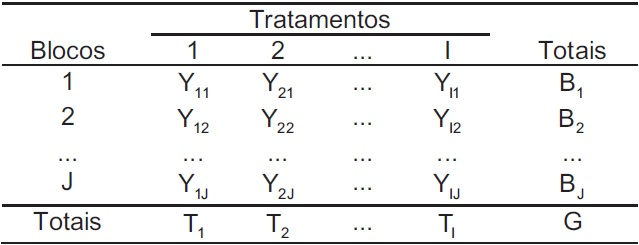
\includegraphics[scale=0.5]{Figuras/Tabulacao}
    %\caption{}
    %\label{figRotulo}
  \end{figure}
\end{block}
\end{frame}

\section{Modelo Estatístico}
\begin{frame}{}
\frametitle{}
\begin{block}{}
\justifying
Para o DBC o modelo estatístico é:
\begin{eqnarray*}
Y_{ij} &=& \mu + t_i + b_j + e_{ij}
\end{eqnarray*}
onde $Y_{ij}$ é o valor esperado para a variável resposta obtido para o i-ésimo tratamento em seu j-ésimo bloco, $\mu$ é a média de todos os valores possíveis da variável resposta, $t_i$ é o efeito do tratamento i no valor observado $Y_{ij}$ dado por $t_i = \mu_i - \mu$, $b_j$ é o efeito do bloco $j$ no valor observado $Y_{ij}$ dado por $b_j = \mu_j - \mu$ e $e_{ij}$ é o erro experimental associado ao valor observado $Y_{ij}$ dado por $e_{ij} = Y_{ij} - \mu - \mu_i - \mu_j$.
\end{block}
\end{frame}

\begin{frame}{}
\frametitle{}
\begin{block}{}
\justifying
Para realizar a análise dos dados obtidos de um experimento instalado segundo o DBC, deve-se decompor a variação total que existe entre todas as observações nas partes que a compõem. Neste tipo de delineamento, a decomposição é feita da seguinte forma:
\begin{eqnarray*}
SQTotal &=& SQTrat + SQBlocos + SQRes,
\end{eqnarray*}
onde tais valores são obtidos a partir das somas de quadrados.
\end{block}
\end{frame}

\begin{frame}{}
\frametitle{}
\begin{block}{}
\justifying
\begin{eqnarray*}
% \nonumber % Remove numbering (before each equation)
  SQTotal &=& \sum_{i,j=1}^{I,J} {Y_{ij}}^2 - \frac{\bigg(\sum_{i,j=1}^{I,J} Y_{ij} \bigg)^2}{IJ} \\
  \\
  SQTrat &=& \sum_{i=1}^{I} \frac{T_i^2}{J} - \frac{\bigg(\sum_{i,j=1}^{I,J} Y_{ij}\bigg)^2}{IJ} \\
  \\
  SQBlocos &=& \sum_{j=1}^{J} \frac{B_j^2}{I} -  \frac{\bigg(\sum_{i,j=1}^{I,J} Y_{ij}\bigg)^2}{IJ}\\
  \\
  SQRes &=& SQTotal - SQTrat - SQBlocos
\end{eqnarray*}

\end{block}
\end{frame}

\section{Análise de Variância}
\begin{frame}{}
\frametitle{}
\begin{block}{}
\justifying
O quadro da ANOVA para a análise de um experimento instalado segundo DBC é do seguinte tipo:
\begin{table}[!h]
\scalebox{0.7}{%
\setlength{\arrayrulewidth}{2pt}
\begin{tabular}{cccccc}
\hline
FV&GL&SQ&QM&F&$F_{tab;\alpha}$\\
\hline
&&&&&\\
Blocos&$(J-1)$&SQBlocos& $-$&$-$&$-$\\
&&&&&\\
Tratamentos&$(I-1)$&SQTrat&$\dfrac{SQTrat}{I-1}$&$\dfrac{QMTrat}{QMRes}$&$[(I-1);(I-1)(J-1)]$\\
&&&&&\\
Resíduo&$(I-1)(J-1)$&SQRes&$\dfrac{SQRes}{(I-1)(J-1)}$&$-$&$-$\\
\hline
Total&IJ-1&SQTotal&$-$&$-$&$-$\\
\hline
\end{tabular}
}
\end{table}
\end{block}
\end{frame}

\begin{frame}{}
\frametitle{}
\begin{block}{}
\justifying
As hipóteses para o teste $F$ da análise de variância para tratamentos são as seguintes:
\begin{itemize}
\item $H_0: \mu_1 = \mu_2 = \cdots = \mu_l$, que equivale a dizer que todos os possíveis contrastes entre as médias dos tratamentos são estatisticamente nulos, ao nível de probabilidade exucutado no teste.
\item $H_1:\ \textrm{não}\ H_0$, que equivale a dizer que existe pelo menos um contraste entre as médias dos tratamentos estatisticamente diferentes de zero, ao nível de probabilidade executado no teste.
\end{itemize}
\end{block}
\end{frame}

\begin{frame}{}
\frametitle{}
\begin{block}{}
\justifying
Para se concluir se existe diferença entre tratamentos, calcula-se o valor esperado $F$, que é obtido pelo quociente do $QMTrat$ com o $QMRes$. Este valor de 
$F$ deve ser comparado com o valor de $F$ tabelado, o qual é obtido na tabela de distribuição do teste $F$, de acordo com o nível de significância do teste, graus 
de liberdade para tratamentos e graus de liberdade para resíduo.
\end{block}
\end{frame}

\begin{frame}{}
\frametitle{}
\begin{block}{}
\justifying
A regra decisória para o teste $F$ é a seguinte:
\begin{itemize}
\item se $F_{cal} \geq F_{tab}$, então rejeita-se $H_0$ e conclui-se que os tratamentos tem efeito diferenciado ao nível de significância em que foi realizado o teste
\item se $F_{cal} < F_{tab}$, então não rejeita-se $H_0$ e conclui-se que os tratamentos têm efeitos iguais ao nível de significância em que foi realizado o teste
\end{itemize}
\end{block}
\end{frame}

\section{Exemplo}
\begin{frame}{}
\frametitle{}
\begin{block}{Exemplo 1 (Exercício 6.1, pág. 57)}
\justifying
Os dados abaixo se referem a um experimento instalado segundo o DBC, em que os tratamentos, 5 produtos comerciais para 
suprir a deficiência de micronutrientes em caprinos, foram fornecidos aos animais os quais foram separados em 3 grupos segundo a idade. Os resultados obtidos, 
expressos em ppm de micronutriente por ml de sangue, foram os seguintes:
\vspace{-0.5cm}
\begin{table}[!h]
\begin{tabular}{ccccccc}
\hline
\multicolumn{7}{c}{Produtos Comerciais}\\
\cline{2-6}
Bloco&1&2&3&4&5&Totais\\
\hline
1&83&86&103&116&132&520\\
2&63&69&79&81&98&390\\
3&55&61&79&79&91&365\\
\hline
Totais&201&216&261&276&321&1275\\
\hline
\end{tabular}
\end{table}
\vspace{-0.5cm}
Pede-se proceder a ANOVA e aplicar o teste de Tukey e Duncan, utilizando o nível de significância de $5\%$.
\end{block}
\end{frame}

\end{document}
